\section{Libspotify Abstraction}
\label{imp:libspotify}
As stated in \cref{techPlat:music_catalog_libspotify} the only way to stream tracks off Spotify is using the C library libspotify. Being written as a C library, one has to take care of managing memory allocation correctly in order to avoid runtime exceptions while using libspotify.

To make it harder to cause these runtime errors and to ease
interoperability in the C\# environment, a C\# library can be written
that abstracts the error prone elements of C programs away. The C\#
library \enquote{SpotifyDotNet} developed for use in the software
described in this paper, does just that. This corresponds to the
SpotifyDotNet component described in \cref{sec:architecture}.

\subsection{Abstracting Low-level C Concepts Away}
\label{libspotify:abstracting_low_level_c_concepts_away}

The goal of the SpofityDotNet library is to minimize runtime exceptions caused by memory related errors. To do this, the error prone unmanaged C code has to be accessed as secure managed C\# code.

SpotifyDotNet uses existing bindings, hosted on \url{http://libspotifydotnet.codeplex.com/}, to interface with libspotify from C\#. As an example let's look at the login function from libspotify. See \cref{fig:loginC}. The corresponding binding can be seen in \cref{fig:loginCsharp}. As can be seen, a C pointer maps directly to an IntPtr struct in C\#. \lstinline|const char*| becomes a common string object in C\#. A C bool is simply a C\# bool.

\begin{lstlisting}[float, floatplacement=htpb,caption = {Libspotify login function prototype - C}, label = {fig:loginC}]
sp_error sp_session_login ( sp_session *session,
                            const char *username,
                            const char *password,
                            bool remember_me,
                            const char *blob
                          )
\end{lstlisting}

\begin{lstlisting}[float, floatplacement=htpb,caption = {Login method using a external implementation from libspotify.dll - C\#}, label={fig:loginCsharp}]
public static extern sp_error sp_session_login ( IntPtr sessionPtr,
                                                 string username,
                                                 string password,
                                                 bool rememberMe,
                                                 string blob
                                               )
\end{lstlisting}

However this is not abstracted enough. To the user of the library, no pointers should be visible. This is solved by encapsulating state and data inside the Spotify class. This class is the entry point to using libspotify in C\#. See \cref{fig:spotifydotnet_class} for complete class diagrams. The main operation on the class is the Login method. This method is asynchronous so it will utilise the C\# feature of Tasks. A Task is simply a promise that something will happen in the future. In this context, the login method returns an \lstinline|Task<Tuple<SpotifyLoggedIn,LoginState>>|. So the login method promises that it will return \lstinline|Tuple<SpotifyLoggedIn,LoginState>| at some time in the future. When login has occurred, LoginState will describe the state of the login process. If LoginState is \enquote{OK}, the login was successful and SpotifyLoggedIn will be non-null. If LoginState was anything other than \enquote{OK}, SpotifyLoggedin would be null. The SpotifyLoggedIn object sent with the login method, exposes all methods that are available when logged into Spotify. See \cref{fig:spotifydotnet_class}. By only exposing the SpotifyLoggedIn object when correctly logged in, certain errors like searching without being logged in, can be detected at compile time.

\begin{figure}[hbtp]
  \centering
  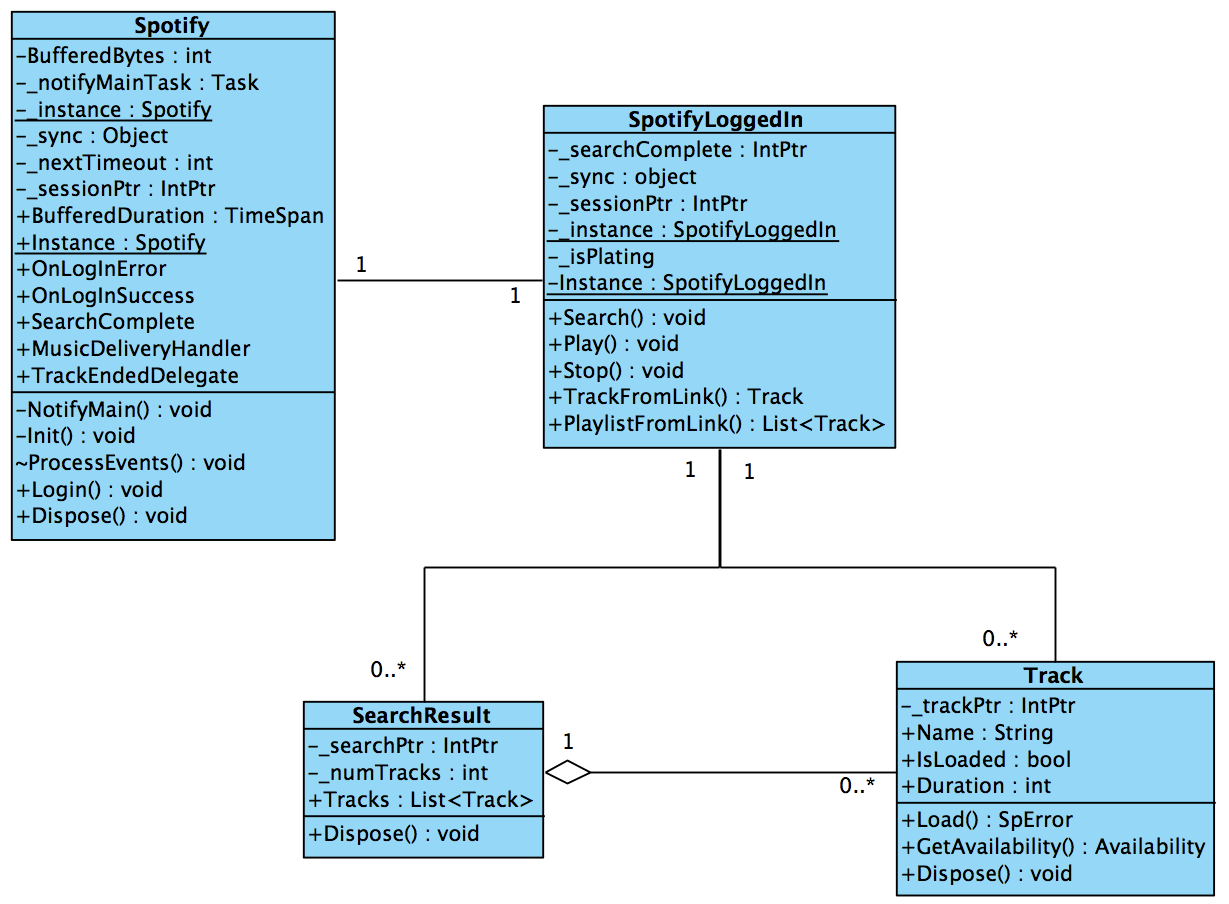
\includegraphics[width=1.2\linewidth]{spotifydotnetClass.png}
  \caption{Class diagram of SpotifyDotNet library.}
  \label{fig:spotifydotnet_class}
\end{figure}

\subsection{Making it Thread-safe}
\label{libspotify:making_it_thread_safe}

Libspotify is not thread safe~\cite{spotifyLibspotifyFAQ}. This is solved in SpotifyDotNet by using locks around non thread safe code. This is easily done in C\# using the \enquote{lock} keyword as seen in \cref{lst:lock_keyword}. Locks are a way to avoid race conditions i.e. threads modifying the same chunk of memory at the same time. Race conditions lead to non-deterministic results, which is always to be avoided. Locks solve this issue by synchronizing the threads. Whatever code blocks are wrapped around locks can only be accessed by one thread at a time.

\begin{lstlisting}[float, floatplacement=htpb, caption = {Example of using the lock keyword in C\#. \enquote{\_sync} is an object used to store the lock state}, label = {lst:lock_keyword}]
lock(_sync) {
  thisWillRunThreadSafe();
}
\end{lstlisting}

To the user of SpotifyDotNet, no errors related to threads can occur when using the library on multiple threads.
